\section{Introduction}

\subsection{Présentation du projet}

Le projet consiste en une solution complète permettant le monitoring à distance de sites géographiquement isolés. L'attention est ici plus particulièrement portée sur le monitoring du niveau de remplissage des cuves. Le but étant de pouvoir à tout moment avoir une vision d'ensemble sur un territoire complet des sites nécessitant une intervention. Une des contraintes de cette solution technique est de pouvoir fonctionner par de très basses températures, et dans des régions où l'éclairement n'est pas garanti (cercle polaire).

\subsection{Présentation du document}

Ce cahier des charges va présenter en détails les exigences relatives à la solution de communication par satellite des sites isolés avec le centrale de gestion, ainsi que la reconfiguration à distance des ceux-ci. Seront d'abord présentés les objectifs de la ce sous-système, les utilisateurs concernés, et les problèmes pouvant se présenter lors de son utilisation, autant dans son développement, que dans sa mise en oeuvre et sa maintenance. Ce document est accompagné d'annexes permettant d'approfondir certains sujets plus techniques sur lesquels s'attarder aurait coûté en clarté.

\subsection{Documents applicables / Documents de référence}

Il peut être intéressant d'avoir pris connaissance de ces documents au préalable pour être mieux à même d'appréhender le contenu de ce cahier des charges.

\begin{itemize}
\item Dossier d'étude de faisabilité.
\item Dossier de spécification technique des besoins.
\item Dossier de conception.
\end{itemize}

En complément de ce document, il peut être utile de consulter le dossier des APIs et Interfaces.

\subsection{Terminologie et abréviations}

\begin{itemize}
\item Système central : Serveur principal de la solution technique. Récupère les données depuis l'ensemble des sites isolés, et permet leur consultation ainsi que de la prise de décisions depuis un portail en ligne.
\item Système de gestion du site isolé : Logiciel ``maître'' de la station. C'est lui qui coordone la récupération des données depuis les capteurs, leur traitement local, et qui va utiliser le système de transmission (que décrit ce document) pour envoyer ces données au système central.
\item Station du site isolé : Point central d'un site, est composée d'un système embarqué, de batteries, et de moyens de communications avec les capteurs, et avec le système central.
\end{itemize}

\begin{itemize}
\item GSM (Global System for Mobile communications) : Technologie dominante de communication sans-fil utilisée par les téléphones portables. 
\item GPRS (General Packet Radio Service) : Service de transfert de données utilisant le GSM. Il permet l'accès au réseau Internet depuis n'importe quel terminal compatible, si l'opérateur le permet.
\item GlobalStar : Opérateur de télécommunications par satellites. Propose une couverture mondiale d'un service de communication voix/données accessible depuis des terminaux spécialisés.
\item TCP (Transmission Control Protocol) : Protocole de communication sur IP garantissant l'intégrité des données transférées.
\end{itemize}

\section{Présentation du problème}

\subsection{Buts, nature du logiciel, utilisateurs concernés}

Cette étude porte sur un composant logiciel qui va s'exécuter aux côtés du système de gestion de site sur le système embarqué de la station du site isolé.

Ce rôle de ce logiciel va être de communiquer avec le système central à l'aide d'une connexion satellite ou GSM. Il aura donc une responsabilité double : d'un côté il assurera la transmission des données que les capteurs auront relevés, de l'autre il pourra recevoir en retour des informations de configuration, qui pourront s'appliquer à ce système, mais aussi à l'ensemble de la station et des capteurs.

En clair, ce système va être le seul moyen de communication du site isolé vers l'extérieur. Il devra pour cela exploiter un module de communication matériel qui sera connecté au système embarqué de la station.

Le composant décrit ici n'aura pas directment d'``utilisateurs'' à proprement parler. Il devra par ailleurs fournir une API aux développeurs du système de gestion du site isolé, et se conformer au protocole utilisé par le système central. La configuration du composant (e.g. les fréquences satellites à utiliser pour la communication) pourra se faire à l'aide d'un fichier de configuration, ou alors à distance, lors de la réception de nouvelles données de configuration.

\subsection{Formulation des besoins, exploitation et ergonomie, expérience}

Le système présenté doit répondre à deux besoins bien distincts, et ce quelque soit la localisation géographique du système dans le monde :

\paragraph{Transmission} Le système doit pouvoir envoyer au système central les informations suivantes :

\begin{itemize}
\item La valeur des mesures effectuées depuis la dernière transmission par chacun des capteurs. La quantité de valeurs dépend de la granularité avec laquelle est configurée le site. Chaque valeur sera bien évidemment horodatée.
\item L'état physique et logique de la station et du site. Cela peut comprendre la température ambiante, l'autonomie estimée des différentes batteries, les logs systèmes engrangés par le système informatique, etc.
\item L'identification du site et des différents capteurs. % A voir.
\end{itemize}

\paragraph{Reconfiguration} Après envoi des données, le système peut éventuellement recevoir comme réponse une demande de reconfiguration permettant aux opérateurs de modifier à distance les paramètres suivants :

\begin{itemize}
\item Les différents quantum de temps définissant la granularité avec laquelle le système effectue ses mesures et en transmet les résultats au système central.
\item Les fréquences de transmission satellite utilisées par le présent sous-système.
\item Des paramètres systèmes tels que le niveau de logs à engranger et à transmettre, les politiques de reprise sur échec (dans le contexte de la communication avec les capteurs par exemple).
\item Des données de configuration spécifiques à certains capteurs, qui leur seront transmis à leur prochaine connexion (les intervalles de relevés comme mentionné plus haut, mais aussi des paramètres spécifiques à un type de capteur tels que les fréquences d'ultrasons à utiliser pour effectuer un relevé de remplissage d'une cuve).
\end{itemize}

Pour permettre un remplacement simplifié, le composant matériel de transmission ne sera pas directement intégré au système embarqué. Il sera connecté à l'aide d'une interface USB standard.

\subsection{Portée, développement, mise en oeuvre, organisation de la maintenance}

Il est indispensable que ce système puisse être maintenu de manière efficace, puisque qu'il est vital au bon fonctionnement de l'intégralité du système de monitoring d'un site isolé. La maintenance portera sur les aspect suivants du système :

\begin{itemize}
\item La remise à zéro du logiciel, et la mise-à-jour de celui-ci.
\item Le remplacement du matériel de communication (satellite ou GSM) en cas de panne. Il faut aussi prévoir une évolution vers un composant plus perfectionné.\footnotemark
\item La reconfiguration du système, pour fonctionner avec des paramètres différents (e.g. les canaux de communication satellite).
\end{itemize}

\footnotetext{Ceci laisse entrevoir la contrainte d'évolutivité du système, que nous verrons plus en détails par la suite.}

La maintenance à proprement parler pourra se faire de deux manières. La première étant une simple reconfiguration à distance du système en utilisation la capacité du système à recevoir de nouveaux paramètres lors de sa communication avec le système central. Ce type de maintenance peut suffire lorsqu'il ne s'agit que d'une modification légére des options du système.

Pour des problèmes plus sérieux, la maintenance sera effectuée sur site, par un technicien qui viendra se connecter directement au système de gestion du site à l'aide d'un ordinateur portable. C'est ce même technicien qui aura pour rôle d'effectuer des modifications materielles en remplacant des composants enfichables (dans le cas présent, le module de communication par satellite) si le besoin venait à se présenter.

Il sera aussi indispensable que les techniciens puissent vérifier le bon fonctionnement du module de communication matériel indépendament du reste de la station. Cela pour confirmer le diagnostique qu'aura pu fournir le logiciel à ce sujet.

\subsection{Limites}

Ce système ne comprend pas l'autre partie de la transmission de données, à savoir le composant serveur de collecte de celles-ci. On se limite donc ici au composant logiciel présent sur le système de gestion d'un site isolé. Un protocole est défini dans le dossier des APIs et Interfaces décrivant la manière dont la communication avec le système central prendra place.

Ce système n'a pas non plus pour rôle de stocker la configuration du système de gestion du site. Il se contente de transmettre de nouvelles valeurs de configuration à celui-ci lorsqu'il en reçoit, à l'aide encore une fois de l'interface décrite dans le dossier des APIs et Interfaces.

\section{Exigences fonctionnelles}

\subsection{Fonctions de base et performances}

Voici les fonctions de base que va devoir assurer le composant logiciel de transmission :

\begin{itemize}
\item Réception des données à transmettre de la part du système de gestion du site.
\item Gestion du périphérique de transmission, à savoir installation et configuration des pilotes, mais aussi son initialisation et sa configuration.
\item Utilisation du périphérique de transmission pour communiquer avec le serveur central. Envoi des données de capteurs dans un sens, réception des informations de configuration dans l'autre.
\item Transmission au système de gestion du site des données de configuration recues du serveur central.
\end{itemize}

Bien évidemment, la transmission se fait de manière périodique, et non pas en continue.

Il n'y a pas de contrainte forte par rapport aux performances de transmission, le volume des données à transmettre étant relativement faible par rapport aux capacité des connexions modernes de type satellite ou GSM. Une vitesse de 128kpbs en émission/réception sera donc suffisante.

Afin de garantir la confidentialité des données transmises, une connexion sécurisée sera nécessaire entre la station et le système central.

\subsection{Contraintes d'utilisation}

Les contraintes viennent principalement de la nature autonome du système. Cela implique d'avoir :

\begin{itemize}
\item Une faible consomation energétique (et si possible, de ne rien consommer la plupart du temps).
\item La capacité à reprendre une transmission sans aucune perte de données en cas de coupure de la connexion ou de redémarrage du système.
\item Un mode de secours essayant de se connecter à des réseaux secondaires en cas de perte totale des capacités de connexion (recherche de satellites différents, d'opérateurs différents).
\end{itemize}

Certaines contraintes vont venir des choix effectués sur les autres composants de la solution technique dans son ensemble. Il faudra donc que le système de communication du site isolé puisse s'exécuter sur un OS Linux, cela a évidemment aussi conditionné le choix du composant matériel.

\subsection{Critères d'appréciation de la réalisation effective de la fonction}

\begin{itemize}
\item Capacité du système à répondre aux besoins spécifiés.
\item Capacité du système à respecter les contraintes d'utilisation.
\item Respect des standards de qualité en conformité avec la norme ISO 9001.
\end{itemize}

\subsection{Flexibilité dans la façon de mettre en oeuvre la fonction concernée, variation de coûts associée en fonction de cette flexibilité}

Un premier aspect de flexibilité de l'implémentation de ce système va venir de l'emplacement où sera situé le site isolé. Selon la localisation de celui-ci, il faudra en effet faire le choix de l'utilisation d'un module matériel de communication satellite, ou alors d'un module GSM. Bien évidement, le premier revient beaucoup plus cher que le second (autant à l'achat, qu'ensuite lors de son exploitation). On s'autorisera une marge de 50\% sur le coût du composant matériel de transmission en fonction de cette contrainte.

Il est aussi possible d'être flexible sur le paramètrage qu'autorisera ce système, car cela dépendra en grande partie du composant matériel choisi, et du réseau/opérateur de télécommunication qui sera utilisé. Selon les cas, on se retrouvera donc avec plus ou moins d'options de configurations.

\section{Exigences non fonctionnelles}

\section{Contraintes imposées, faisabilité technologique, moyens}

Pour faciliter l'évolutivité future du système, nous avons les contraintes non fonctionnelles suivantes :

\begin{itemize}
\item Modularité extrème du logiciel (pour remplacer n'importe quel bloc sans avoir à toucher aux autres).
\item Indépendance maximum par rapport au composant matériel. Il sera ainsi aisé de passer d'un type de communication (satellite) à l'autre (GSM).
\item Respect des conventions d'architecture et de style décidées au préalable. La production continue de documentation sera aussi exigée.
\end{itemize}

\subsection{Sûreté}

Comme mentionné à plusieurs reprises dans ce document, il est capital que la transmission de données se fasse de manière sûre et fiable. Pour cela, nous proposons l'utilisation de la technologie HTTPS pour la communication entre la station et le système central, et ce pour les raisons suivantes :

\begin{itemize}
\item Basé sur le protocole TCP, cette technologie assure l'intégrité des données transmises.
\item Le cryptage de la connexion, basé sur le RSA, n'a plus à faire ses preuves, et est simple à mettre en oeuvre.
\item L'utilisation du protocole HTTP permet de grandement faciliter l'implémentation et le développement du système central.
\end{itemize}

Pour plus de précisions sur la manière dont communiqueront ce système et le système central, consulter le dossier des APIs et Interfaces.

\subsection{Complexité}

L'insistance sur l'utilisation de protocoles et techniques de communication standard assure que la complexité à ce niveau reste dans des limites acceptables. En revanche, c'est au niveau de la communication avec le composant matériel qu'il faut s'adapter à l'API proposée en se basant sur la documentation constructeur, c'est donc là que résidera le gros de la complexité de l'implémentation du système.

\subsection{Compétences}

Compétences nécessaires à la réalisation du projet :

\begin{itemize}
\item Expertise en modules électroniques.
\item Programmation linux bas-niveau.
\item Expertise en protocoles et sécurité réseau.
\end{itemize}

\subsection{Normes de documentation}

Les normes de documentation à adopter sont décrites dans le plan d'assurance qualité commun aux différents éléments de ce projets.

\section{Configuration cible}

\subsection{Matériels et logiciels}

Selon la configuration séléctionnée, le module matériel utilisé l'un des deux suivants :

\paragraph{Module PCI Express GTM669WFS}

Ce composant permet de se connecter à n'importe quel réseau GSM. Interfacé simplement en PCIe, ce modem permet de communiquer en utilisant le protocole GPRS en utilisant le réseau d'un opérateur de téléphonie local, il suffit pour cela de lui adjoindre la carte SIM adaptée.

\paragraph{Modem Satellite GSP-1720}

Ce modem permet de se connecter au réseau de satellite GlobalStar et assure ensuite une connexion de données en full-duplex. Bien plus coûteux que le module GSM, une connexion satellite peut s'avérer nécéssaire pour certains lieux très isolés.

Pour plus d'information sur ces composants, se reporter aux annexes.

Au niveau du logiciel, le système devra pouvoir s'exécuter sur le même OS embarqué Linux que le système de gestion du site.

\subsection{Stabilité de la configuration}

Pour des raisons d'évolutivité, le système devra pouvoir s'adapter facilement à un remplacement du composant matériel, et éventuellement à un remplacement de celui-ci par un autre modèle (dans le cas où le besoin se présenterait d'utiliser un autre opérateur de télécommunications par exemple).

L'accent devra donc être mis lors de la phase de développement logiciel sur la modularité afin de limiter l'effort de maintenance dans le cas où il faudrait adapter le logiciel à un nouveau matériel, mais aussi à de nouveaux protocoles de communication avec les autres briques de la solution.

\subsection{Description des API}

Le système va communiquer avec les autres composants de la solution de monitoring de sites isolés de deux manières différentes :

\paragraph{API d'envoi et de réception de données}

Cette API est destinée au système de gestion du site, et va permettre à celui-ci de transmettre à notre logiciel les données relevées par les capteurs. Elle expose les méthodes suivantes :

\begin{itemize}
\item GetStatus : Permet de connaitre l'état actuel du système de transmission. S'il est actuellement en cours de transmission de données, ou si des données sont en attente d'envoi pour plus tard. Permet aussi de savoir quand le transfert est terminé.
\item GetFullStatus : Permet d'obtenir un diagnostique complet de l'état du système. Ce aussi bien au niveau logiciel que matériel. Cette méthode sera utile pour les techniciens qui seront amenés à effectuer des maintenances sur le système.
\item SendData : Prend en paramètre le fichier à transmettre, sous forme binaire. Le système essayera de transmettre ces données dès qu'il le pourra, et peut mettre en attente plusieurs fichiers qu'il enverra plus tard.
\item GetData : Dans le cas où des données de configuration ont été reçues, elles seront disponibles par le biais de cette méthode.
\end{itemize}

\paragraph{Protocole de communication avec le serveur central}

La communication avec le serveur central s'effectue à l'aide d'un protocole HTTP Restful\footnotemark. Les détails de l'API serveur et du protocole utilisé seront disponibles dans le dossier des APIs et Interfaces.

\footnotetext{``Representational State Transfer'' : Principes définissant une organisation standard pour une API web.}

\section{Guide de réponse au cahier des charges}

Tests unitaires :

\begin{itemize}
\item Test de l'interface matérielle avec le module matériel de communication.
\item Test de l'interface logicielle avec le système de gestion du site.
\item Test du protocole de communication avec le système central.
\item Test de communication GPRS/Satellite.
\end{itemize}

Tests d'intégration :

\begin{itemize}
\item Test de reprise après arret spontanné du système.
\item Test de reprise du transfert en cas de coupure de la connexion.
\end{itemize}

\newpage
\appendix
\appendixpage

\section{GTM669WFS}

\begin{figure}[H]
\subfloat{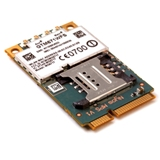
\includegraphics[width=1.5in]{Transmission/Modem3G_1.jpg}}
\label{fig:3g}
\end{figure}

\subsection{Description}

Carte PCI Express de petite taille permettant de se connecter à des réseaux GSM. Dispose en outre d'un récepteur GPS et d'un port MicroSD, et a l'avantage d'avoir un emplacement pour carte SIM, rendant sa configuration plus aisée.

\subsection{Specifications physiques}

\begin{tabular}{|c|c|}
\hline Form factor & PCI Express Mini Card \\ 
\hline Dimensions & 51 x 30 x 4.2 mm \\ 
\hline Poids & 10g \\
\hline Température de fonctionnement & -10°C à +55°C \\
\hline Humidité de fonctionnement & 10 - 90\% RH \\
\hline
\end{tabular} 

\subsection{Connectivité}

Vitesses de connection maximum.

\begin{tabular}{|c|c|c|}
\hline Mode & Débit descendant & Débit montant \\
\hline GSM & 14.4 Kbps & 14.4 Kbps \\
\hline GPRS & 85.6 Kbps & 85.6 Kbps \\
\hline EDGE & 236.8 Kbps & 236.8 Kbps \\
\hline UMTS & 384 Kbps & 384 Kbps \\
\hline HSDPA/HSUPA & 14.4 Mbps & 5.76 Mbps \\
\hline
\end{tabular}

\newpage
\section{GSP-1720}

\setcounter{subfigure}{0}
\begin{figure}[H]
\subfloat[Carte]{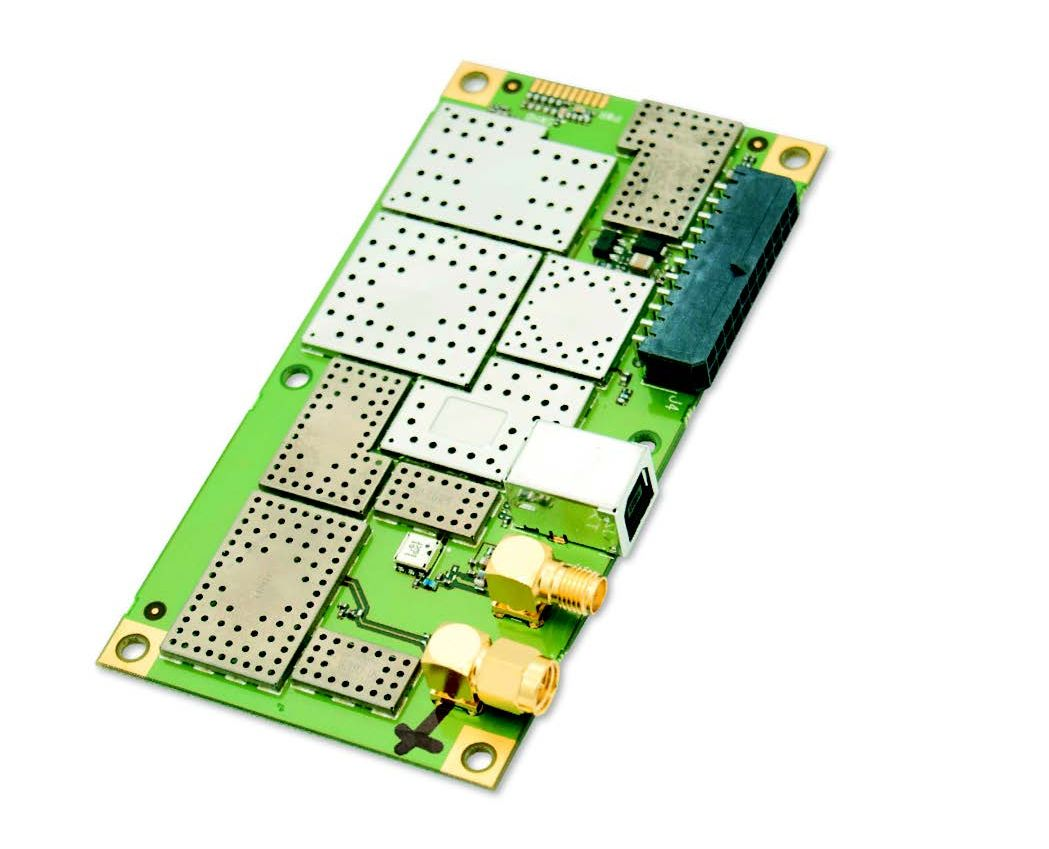
\includegraphics[width=3in]{Transmission/ModemSatellite_1.jpg}}
\subfloat[Antenne]{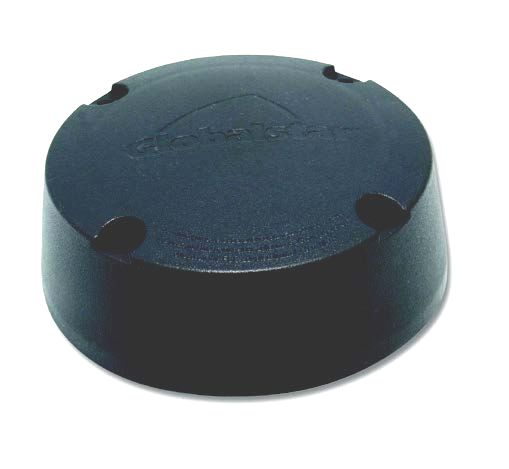
\includegraphics[width=2in]{Transmission/ModemSatellite_2.jpg}}
\label{fig:satellite}
\end{figure}

\subsection{Description}

Ce composant permet une connexion au réseau de télécommunications par satellite GlobalStar. Il supporte les échanges de données en mode duplex, et permet une connexion directe à internet. Son interfacage se faisant en USB, cela ne pose pas de problème pour l'intégration dans le système de transmission.

\subsection{Spécifications physiques}

\begin{tabular}{|c|c|}
\hline Dimensions & 119 x 65 x 15 mm \\
\hline Poids & 60g \\
\hline Fréquences opérationnelles & 
En transmission : 1610 MHz – 1626.5 MHz \\
& En réception : 2483.5 MHz – 2500 MHz \\
\hline Puissance maximum & +31dBm (antenne passive), +34 dBm (antenne active) \\
\hline Consommation electrique à 5V DC & A l'arret : 0.65mW \\
& En veille : 0.5 W \\
& En transmission : 3.65 W \\ 
\hline Températures de fonctionnement & -30 à +60ºC \\
\hline Humidité de fonctionnement & 5 - 95\% RH \\
\hline
\end{tabular}